\documentclass{beamer}\usepackage{graphicx, color}
%% maxwidth is the original width if it is less than linewidth
%% otherwise use linewidth (to make sure the graphics do not exceed the margin)
\makeatletter
\def\maxwidth{ %
  \ifdim\Gin@nat@width>\linewidth
    \linewidth
  \else
    \Gin@nat@width
  \fi
}
\makeatother

\IfFileExists{upquote.sty}{\usepackage{upquote}}{}
\definecolor{fgcolor}{rgb}{0.2, 0.2, 0.2}
\newcommand{\hlnumber}[1]{\textcolor[rgb]{0,0,0}{#1}}%
\newcommand{\hlfunctioncall}[1]{\textcolor[rgb]{0.501960784313725,0,0.329411764705882}{\textbf{#1}}}%
\newcommand{\hlstring}[1]{\textcolor[rgb]{0.6,0.6,1}{#1}}%
\newcommand{\hlkeyword}[1]{\textcolor[rgb]{0,0,0}{\textbf{#1}}}%
\newcommand{\hlargument}[1]{\textcolor[rgb]{0.690196078431373,0.250980392156863,0.0196078431372549}{#1}}%
\newcommand{\hlcomment}[1]{\textcolor[rgb]{0.180392156862745,0.6,0.341176470588235}{#1}}%
\newcommand{\hlroxygencomment}[1]{\textcolor[rgb]{0.43921568627451,0.47843137254902,0.701960784313725}{#1}}%
\newcommand{\hlformalargs}[1]{\textcolor[rgb]{0.690196078431373,0.250980392156863,0.0196078431372549}{#1}}%
\newcommand{\hleqformalargs}[1]{\textcolor[rgb]{0.690196078431373,0.250980392156863,0.0196078431372549}{#1}}%
\newcommand{\hlassignement}[1]{\textcolor[rgb]{0,0,0}{\textbf{#1}}}%
\newcommand{\hlpackage}[1]{\textcolor[rgb]{0.588235294117647,0.709803921568627,0.145098039215686}{#1}}%
\newcommand{\hlslot}[1]{\textit{#1}}%
\newcommand{\hlsymbol}[1]{\textcolor[rgb]{0,0,0}{#1}}%
\newcommand{\hlprompt}[1]{\textcolor[rgb]{0.2,0.2,0.2}{#1}}%

\usepackage{framed}
\makeatletter
\newenvironment{kframe}{%
 \def\at@end@of@kframe{}%
 \ifinner\ifhmode%
  \def\at@end@of@kframe{\end{minipage}}%
  \begin{minipage}{\columnwidth}%
 \fi\fi%
 \def\FrameCommand##1{\hskip\@totalleftmargin \hskip-\fboxsep
 \colorbox{shadecolor}{##1}\hskip-\fboxsep
     % There is no \\@totalrightmargin, so:
     \hskip-\linewidth \hskip-\@totalleftmargin \hskip\columnwidth}%
 \MakeFramed {\advance\hsize-\width
   \@totalleftmargin\z@ \linewidth\hsize
   \@setminipage}}%
 {\par\unskip\endMakeFramed%
 \at@end@of@kframe}
\makeatother

\definecolor{shadecolor}{rgb}{.97, .97, .97}
\definecolor{messagecolor}{rgb}{0, 0, 0}
\definecolor{warningcolor}{rgb}{1, 0, 1}
\definecolor{errorcolor}{rgb}{1, 0, 0}
\newenvironment{knitrout}{}{} % an empty environment to be redefined in TeX

\usepackage{alltt}
\usetheme{Stats}
\setbeamercovered{transparent}
\usepackage{color}
\usepackage{hyperref}
  \hypersetup{
  	colorlinks=true
		linkcolor=black
		}
\usepackage{url}
\usepackage{graphics}
\usepackage{tikz}
\usepackage{booktabs}





%%%%%%%%%%%%%%%%%%%%%%%%%%%%%%%% Title Slide %%%%%%%%%%%%%%%%%%%%%%%%%%
\title[]{Intro to Social Science Data Analysis \\[1cm] Lecture 5: Descriptive Statistics}
\author[]{
    \href{mailto:gandrud@yonsei.ac.kr}{Christopher Gandrud}
}
\date{\today}


\begin{document}

\frame{\titlepage}

\section[Outline]{}
\frame{\tableofcontents}

%%%%%%%%%%%%%%%%%% Recap %%%%%%%%%%%%%%%%%%

\frame{
  \frametitle{Make Up Class}
  {\Large{We need to decide a time to have a make up class. \\[0.5cm]
  The purpose of the class will be to give you a chance to get started on Assignment 2.}}
}

\section{Recap}
\frame{
	\frametitle{Review Questions 1}
  \begin{itemize}
    \item What is reproducible research?
    \item Why is it important?
  \end{itemize}
}

\frame{
  \frametitle{Review Questions 2}
  \begin{itemize}
    \item What is the Markdown markup language?
    \item What does the {\emph{knitr}} package do?
  \end{itemize}
}

\frame{
  \frametitle{Review Questions 3}
  \begin{itemize}
    \item What is a code chunk?
    \item How do you make a code chunk in a Markdown document?
  \end{itemize}
}

\section{Assignment 2}
\frame{
  \frametitle{Assignment 2}
  \textbf{Due:} Friday 19 October \\[0.25cm]
  
  \textbf{Describe} at least \textbf{3} variables in a data set.\\[0.25cm]
  {\small{
    You need to select a \textbf{range of descriptive statistical tools}. The tools should include both \textbf{numerical descriptive statistics} and \textbf{graphics}.\\[0.25cm]

    These tools should describe the variables':
    \begin{itemize}
      \item<1-> central tendency,
      \item<1-> variation,
      \item<1-> their relationships with the other variables.
    \end{itemize}

    The descriptions need to be discussed \textbf{in paragraph form}. \\[0.25cm]

    The description must be \textbf{reproducible}. So you should email me the link to a Dropbox folder with:
    \begin{itemize}
      \item<1-> the \texttt{.csv} data set,
      \item<1-> the \texttt{.Rmd} R markdown file,
      \item<1-> the final \texttt{.html} file.
    \end{itemize}
  }}
}

%%%%%%%%%%%%%%%%%% Describing Data Overall %%%%%%%%%%%%%%%%%%
\section{Describing Data Overall}
\frame{
  \begin{center}
    {\LARGE{So far we have learned how to gather data and get it into R.}}
  \end{center}
}

\frame{
  \begin{center}
    {\LARGE{Today we will start to learn tools for {\bf{describing}} our data.}} \\[0.5cm]
    We will learn {\bf{descriptive statistics}}.
  \end{center}
}

\frame{
  \begin{center}
    {\LARGE{Why do we need tools for describing our data?}}
  \end{center}
}

\frame{
  \frametitle{Why do we need tools for describing our data?}
  \begin{itemize}
    \item To find the {\bf{patterns}} we are interested but too difficult to find by just looking at the raw data.
    \item Find potential {\bf{data biases}}.
  \end{itemize}
}

\frame{
  \begin{center}
    {\LARGE{Always look at the descriptive statistics before starting your data analysis.}}
  \end{center}
}

\frame{
  \frametitle{Key Principles}
  {\LARGE{When describing data, {\bf{ALWAYS}} look at {\bf{BOTH}}}} \\[0.5cm]
  \begin{itemize}
    \item The Central Tendency,
    \item The Variability (dispersion).
  \end{itemize}
}

\frame{
  \frametitle{Central Tendency}
  {\LARGE{Central Tendency}} \\[0.5cm]
  The central value around which the data clusters. \\[0.5cm]
  Examples of descriptive statistics for the central tendency include: the mode, median, and mean (average).
}

\frame{
  \frametitle{Variability}
  {\LARGE{Variability}}
  How the values vary around the central tendency.\\[0.5cm]
  Examples of descriptive statistics for the variability include: the range, interquartile range, standard deviation.
}

%%%%%%%%%%%%%%%%%%%%% Describing Numerical Data %%%%%%%%%%%%%%%%%%%
\section{Describing Numerical Data}
\frame{
  \begin{center}
    {\LARGE{Describing Numerical Data}}
  \end{center}
}

\frame{
  \frametitle{Measurement Level \& Describing Numerical Data}
  Data that is at the {\bf{highest measurment level}} (numerical continuous) can be described using {\bf{all}} of the descriptive statistics.
}

\frame{
  \frametitle{Populations, Samples, and Descriptive Statistics}
  Remember that our data is a {\bf{sample}} of the {\bf{population}}. \\[0.5cm]
  {\bf{Today}} we are going to be describing {\bf{samples}}. \\[0.5cm]
  From week 7 we will start to use statisics that help us {\bf{infer}} things from our samples about the population.
}

\begin{frame}[fragile]
  \frametitle{The Data}
  Most of the examples for this section use World Bank data for 2009 on:
  \begin{itemize}
    \item GDP per capita (current US\$)
    \item Mortality rate, infant (per 1,000 live births)
    \item World Bank region classification
    \item World Bank income level classification
  \end{itemize} \\[0.3cm]
  The sample includes 199 jurisdictions.
\end{frame}

\begin{frame}[fragile]
  You can get the data set using the source code file at: \url{http://bit.ly/OTWEGS} \\[0.5cm]
  You can actually run this source code directly from R using the \texttt{source\_url} command in the {\emph{devtools}} package.
\end{frame}

\begin{frame}[fragile]
\begin{knitrout}
\definecolor{shadecolor}{rgb}{0.969, 0.969, 0.969}\color{fgcolor}\begin{kframe}
\begin{alltt}
\hlcomment{# Load package}
\hlfunctioncall{library}(devtools)

\hlcomment{# Gather data using source code at:}
\hlcomment{# http://bit.ly/OTWEGS}

\hlcomment{# Data is stored in a data frame: MortalityGDP}
\hlfunctioncall{source_url}(\hlstring{"http://bit.ly/OTWEGS"})

\hlcomment{# See contents of MortalityGDP}
\hlfunctioncall{names}(MortalityGDP)
\end{alltt}
\begin{verbatim}
## [1] "country"         "GDPperCapita"   
## [3] "InfantMortality" "region"         
## [5] "income"
\end{verbatim}
\end{kframe}
\end{knitrout}

\end{frame}

\begin{frame}[fragile,plain]
\begin{knitrout}
\definecolor{shadecolor}{rgb}{0.969, 0.969, 0.969}\color{fgcolor}\begin{kframe}
\begin{alltt}
\hlcomment{# Create scatterplot of GDP/Capita & Infant Mortality}
\hlfunctioncall{plot}(MortalityGDP$GDPperCapita,
     MortalityGDP$InfantMortality)
\end{alltt}
\end{kframe}

{\centering 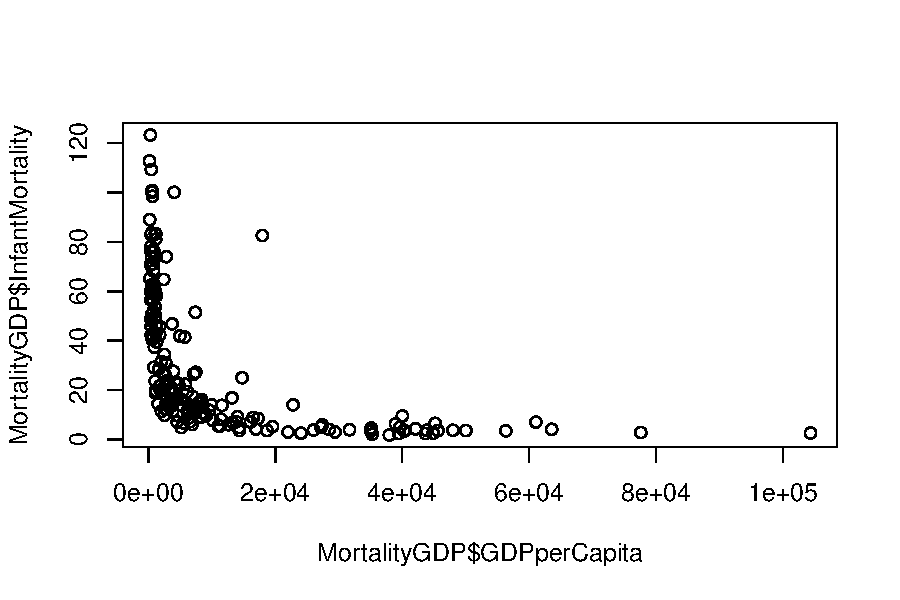
\includegraphics[width=\maxwidth]{figure/Scatter1} 

}


\end{knitrout}

\end{frame}

\frame{
  \frametitle{Central Tendency 1: Mode}
  {\LARGE{Mode}} \\[0.5cm]
  The most common value in a distribution. \\[0.5cm]
  One way to find the mode of a numeric continuous variable is with a {\bf{histogram}}. \\[0.5cm]
  In R you can use the \texttt{hist} command.
}

\begin{frame}[fragile,plain]
\begin{knitrout}
\definecolor{shadecolor}{rgb}{0.969, 0.969, 0.969}\color{fgcolor}\begin{kframe}
\begin{alltt}
\hlfunctioncall{hist}(MortalityGDP$InfantMortality)
\end{alltt}
\end{kframe}

{\centering 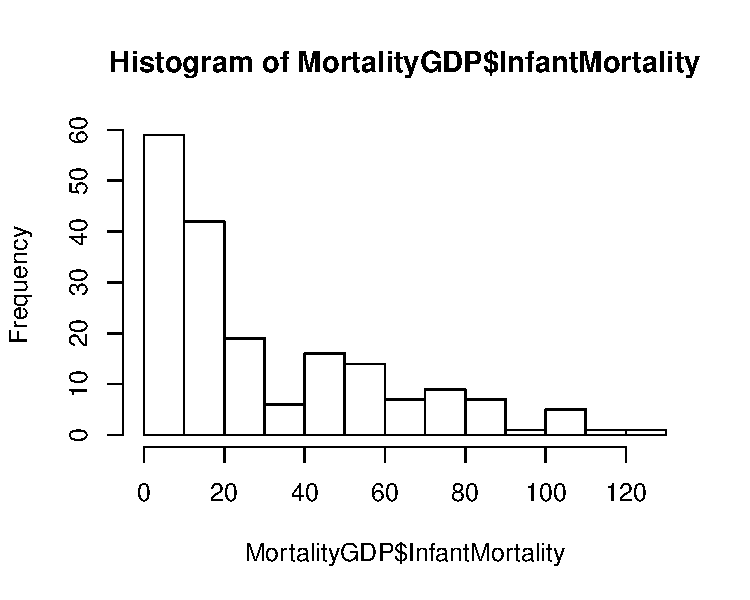
\includegraphics[width=\maxwidth]{figure/InfantHist} 

}


\end{knitrout}

\end{frame}

\frame{
  \frametitle{Uni, Bi, and Multi Modal Distributions}
  A distribution can have {\bf{multiple modes}}.
  \begin{center}
    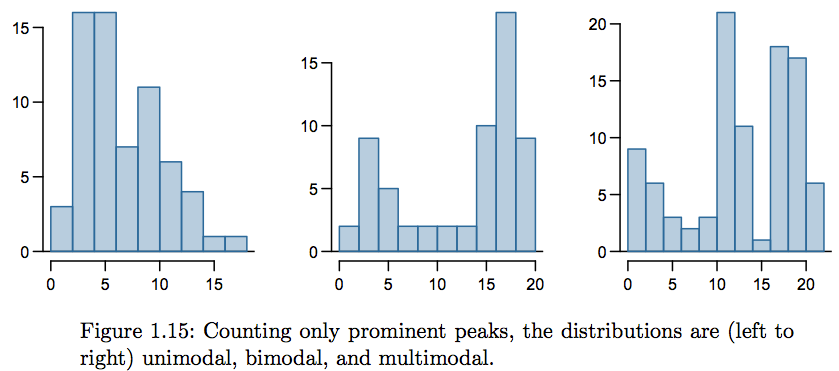
\includegraphics[scale = 0.35]{MultiModal.png} \\[0.75cm]
    {\small{Diez (2011, 12)}}
  \end{center}
}

\begin{frame}[fragile]
  \frametitle{Central Tendency 2: Median}
  {\LARGE{Median}} \\[0.5cm]
  The middle value of a distribution. \\[0.5cm]
  You can find the median with the \texttt{median} command.
\end{frame}  

\begin{frame}[fragile]
\begin{knitrout}
\definecolor{shadecolor}{rgb}{0.969, 0.969, 0.969}\color{fgcolor}\begin{kframe}
\begin{alltt}
\hlcomment{# Create data with no missing values of infant mortality}
InfantNoMiss <- \hlfunctioncall{subset}(MortalityGDP, 
                           !\hlfunctioncall{is.na}(InfantMortality))

\hlcomment{# Find the median infant morality rate}
\hlfunctioncall{median}(InfantNoMiss$InfantMortality)
\end{alltt}
\begin{verbatim}
## [1] 17.2
\end{verbatim}
\end{kframe}
\end{knitrout}

\end{frame}

\begin{frame}[fragile]
  \frametitle{Central Tendency 3: Mean}
  {\LARGE{Mean (average)}} \\[0.5cm]
  The sum of all data values ($x$) divided by the number of data valuse ($n)$. \\[0.25cm]
  {\bf{Population Mean ($\mu_{x}$)}}
  \[
    \mu_{x} = \frac{\sum x}{n}
  \]
  {\bf{Sample Mean ($\bar{x}$)}}
  \[
    \bar{x} = \frac{\sum x}{n}
  \]
\end{frame}

\begin{frame}[fragile]
  You can find the mean with the \texttt{mean} command.
\begin{knitrout}
\definecolor{shadecolor}{rgb}{0.969, 0.969, 0.969}\color{fgcolor}\begin{kframe}
\begin{alltt}
\hlcomment{# Find the mean of InfantMortality}
\hlfunctioncall{mean}(InfantNoMiss$InfantMortality)
\end{alltt}
\begin{verbatim}
## [1] 30.23
\end{verbatim}
\end{kframe}
\end{knitrout}

\end{frame}

\begin{frame}[fragile]
  \frametitle{What is the Central Tendency of Infant Mortality?}
  {\Large{What is the Central Tendency of Infant Mortality?}} \\[0.5cm]
  \begin{itemize}
    \item {\bf{Mode:}} 0-10
    \item {\bf{Median:}} 17.2
    \item {\bf{Mean:}} 30.2
  \end{itemize}
\end{frame}

\frame{
  \frametitle{Skewed}
  {\Large{The reason that these three measures of central tendency are {\bf{not the same}} is that the distribution of Infant Mortality in the sample is {\bf{highly skewed}}.}}
}

\frame{
  \frametitle{Normally Distributed}
  {\Large{Data that is {\bf{normally distributed}} has the same mode, median, and mean. \\[0.5cm]
  Normally distributed data also is {\bf{not skewed}}. It has the same variance on the right and left of the central tendency.}}
}

\begin{frame}[fragile,plain]
\begin{knitrout}
\definecolor{shadecolor}{rgb}{0.969, 0.969, 0.969}\color{fgcolor}\begin{kframe}
\begin{alltt}
\hlcomment{# Simulate normally distributed data}
Normal <- \hlfunctioncall{rnorm}(1e+05, mean = 50, sd = 10)
\end{alltt}
\end{kframe}
\end{knitrout}


\begin{knitrout}
\definecolor{shadecolor}{rgb}{0.969, 0.969, 0.969}\color{fgcolor}

{\centering 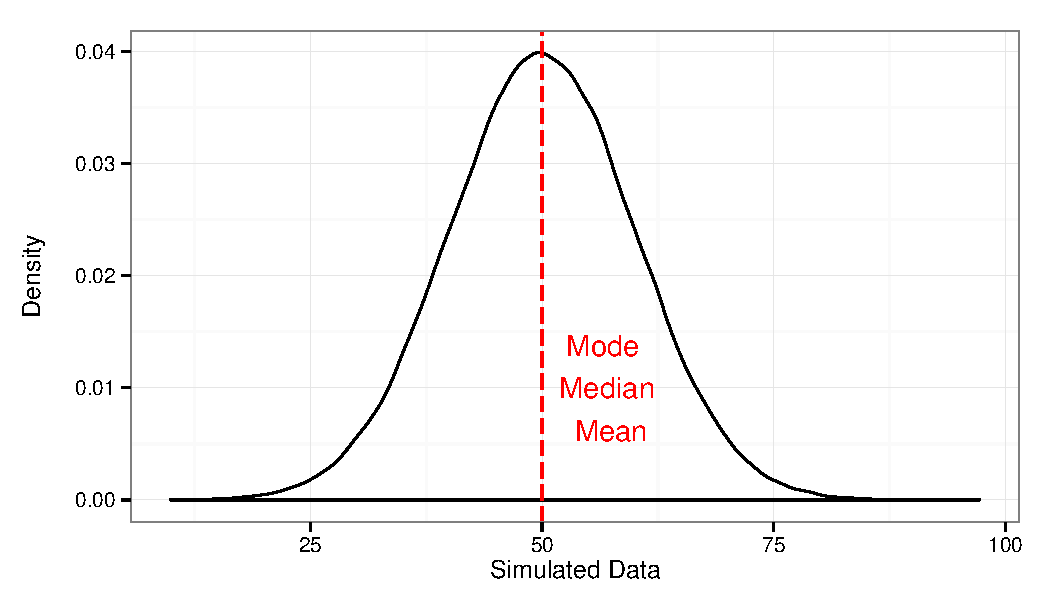
\includegraphics[width=\maxwidth]{figure/NormallyDistGraph} 

}


\end{knitrout}

\end{frame}

\begin{frame}[fragile]
  \frametitle{}
  {\Large{The Infant Mortality data is very right skewed.}}
\begin{knitrout}
\definecolor{shadecolor}{rgb}{0.969, 0.969, 0.969}\color{fgcolor}

{\centering 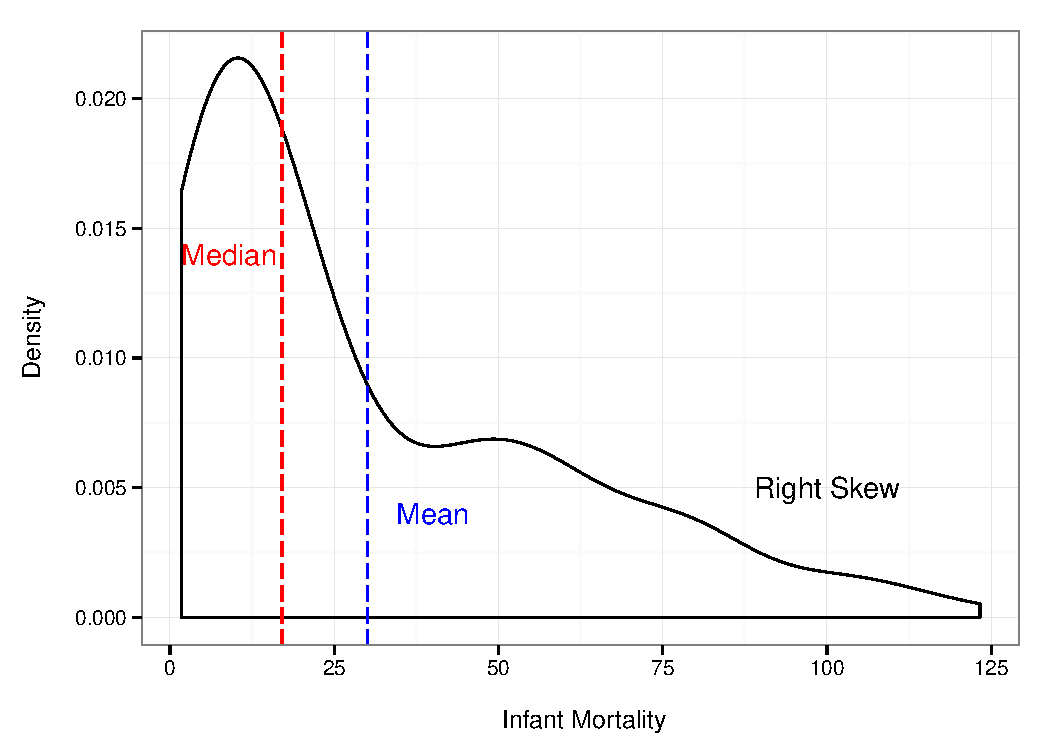
\includegraphics[width=\maxwidth]{figure/HistoAgain} 

}


\end{knitrout}

\end{frame}

\frame{
  \frametitle{Describing Skewness}
  {\Large{A distribution can be:}}
  \begin{itemize}
    \item Right skewed (positively skewed)
    \begin{itemize}
      \item Right skewed data pulls the mean up.
    \end{itemize}
    \item Left skewed (negatively skewed)
    \begin{itemize}
      \item Left skewed data pulls the mean down.
    \end{itemize}
  \end{itemize}
}

\frame{
  \frametitle{Why Variability}
  {\LARGE{So, the central tendency does not adequately describe distributions by itself. \\[0.5cm]
  We also need descriptive statistics of the {\bf{variability}}}}
}

\begin{frame}[fragile]
  \frametitle{Variability 1: Range}
  {\LARGE{Range}} \\[0.5cm]
  The range is the simplest way to describe variability. \\[0.5cm]
  It is the lowest and highest value. \\[0.5cm]
  We can find the range with the \texttt{range} command.
\begin{knitrout}
\definecolor{shadecolor}{rgb}{0.969, 0.969, 0.969}\color{fgcolor}\begin{kframe}
\begin{alltt}
\hlfunctioncall{range}(InfantNoMiss$InfantMortality)
\end{alltt}
\begin{verbatim}
## [1]   1.8 123.3
\end{verbatim}
\end{kframe}
\end{knitrout}

\end{frame}

\begin{frame}[fragile]
  \frametitle{Variability 1: Range}
  {\LARGE{Problems with the Range}} \\[0.5cm]
  The range is highly influenced by {\bf{outliers}}--extreme values. \\[0.5cm]
  It also {\bf{ignores}} all of the data between the minimum and maximum values.
\end{frame}

\begin{frame}[fragile,plain]
\begin{knitrout}
\definecolor{shadecolor}{rgb}{0.969, 0.969, 0.969}\color{fgcolor}\begin{kframe}
\begin{alltt}
\hlcomment{#### Find infant mortality outliers }
\hlcomment{# Reorder data based on infant mortality}
OrderMort <- InfantNoMiss[
                      \hlfunctioncall{order}(InfantNoMiss$InfantMortality,
                            decreasing = TRUE), ]
\hlcomment{# Keep country & InfantMortality}
OrderMort <- OrderMort[, \hlfunctioncall{c}(\hlstring{"country"},
                          \hlstring{"InfantMortality"})]

\hlcomment{# Show high values}
\hlfunctioncall{head}(OrderMort)
\end{alltt}
\begin{verbatim}
##                      country InfantMortality
## 187             Sierra Leone           123.3
## 38          Congo, Dem. Rep.           112.8
## 39  Central African Republic           109.3
## 190                  Somalia           108.3
## 134                     Mali           100.8
## 12                    Angola           100.1
\end{verbatim}
\end{kframe}
\end{knitrout}

\end{frame}

\begin{frame}[fragile]
  \frametitle{Variability 1: Interquartile Range}
  {\LARGE{Interquartile Range}} \\[0.5cm]
  One way to deal with outliers is to look at the interquartile range. \\[0.25cm]
  The interquartile range is the difference between the upper and lower quartiles. \\[0.25cm]
  A quartile is 25\% of the data. \\[0.25cm]
  The {\bf{lower quartile}} is the point up to the lower 25\% of the data.
  The {\bf{upper quartile}} is the point up to the upper 75\% of the data.

\end{frame}

\begin{frame}[fragile]
\begin{knitrout}
\definecolor{shadecolor}{rgb}{0.969, 0.969, 0.969}\color{fgcolor}\begin{kframe}
\begin{alltt}
\hlcomment{# Find what the quartile points are}
\hlfunctioncall{summary}(InfantNoMiss$InfantMortality)
\end{alltt}
\begin{verbatim}
##    Min. 1st Qu.  Median    Mean 3rd Qu.    Max. 
##     1.8     7.2    17.2    30.2    49.0   123.0
\end{verbatim}
\end{kframe}
\end{knitrout}


\[
  48.92 - 7.175 =  
\]

\begin{knitrout}
\definecolor{shadecolor}{rgb}{0.969, 0.969, 0.969}\color{fgcolor}\begin{kframe}
\begin{alltt}
\hlcomment{# Find the interquartile range of InfantMortality}
\hlfunctioncall{IQR}(InfantNoMiss$InfantMortality)
\end{alltt}
\begin{verbatim}
## [1] 41.85
\end{verbatim}
\end{kframe}
\end{knitrout}

\end{frame}

\begin{frame}[fragile,plain]
\begin{knitrout}
\definecolor{shadecolor}{rgb}{0.969, 0.969, 0.969}\color{fgcolor}\begin{kframe}
\begin{alltt}
\hlcomment{# Boxplot showing interquartile range}
\hlfunctioncall{boxplot}(InfantNoMiss$InfantMortality,
        main = \hlstring{"Boxplot of Infant Mortality"})
\end{alltt}
\end{kframe}

{\centering 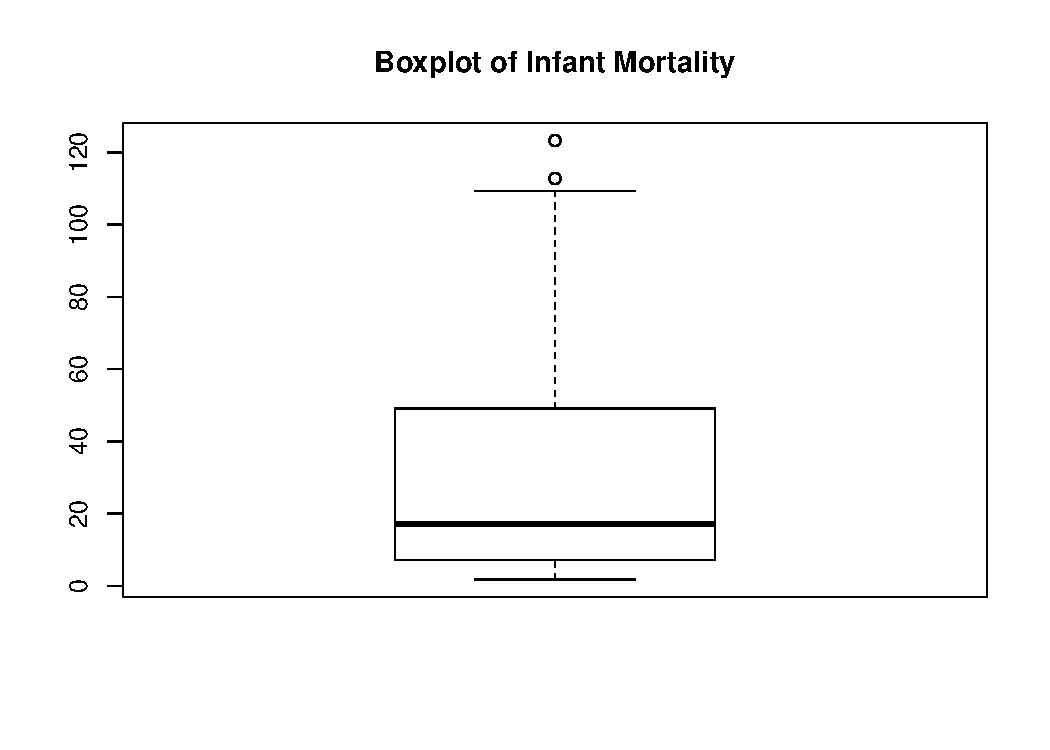
\includegraphics[width=\maxwidth]{figure/BoxPlot} 

}


\end{knitrout}

\end{frame}

\frame{
  \frametitle{More Information on Boxplots}
  {\LARGE{See Diaz (2011, 16) for more boxplot details.}}
}

\frame{
  \frametitle{}
  {\LARGE{A bigger range means {\bf{more variablity}}. \\[0.5cm]
  Note: big in terms of the variable's scale.}}
}

\frame{
  \frametitle{Variability 3: Standard Deviation}
  {\LARGE{Standard Deviation}}. \\[0.5cm]
  The interquartile range describes variation in terms of the median. \\[0.5cm]
  The standard deviation describes {\bf{variation in terms of the mean}}.
}

\frame{
  \frametitle{What is the Sample Standard Deviation? (1)}
  {\Large{The standard deviation is made of the following parts.}} \\[0.25cm]
  {\bf{Deviation}}: the distance of an observation $x$ from the mean $\bar{x}$. 
  \[
    \mathrm{Deviation} = x - \bar{x}  
  \]
  {\bf{Sum of Squares}}: the sum of the squared deviations (they have to be squared or the sum will $= 0$)
  \[
    \mathrm{Sum\:of\:Squares} = \sum(x - \bar{x})^{2}
  \]
  {\bf{Degrees of Freedom}}: Sample size $n$ minus the number of parameters. Today the number of parameters $= 1$. {\small{(See Crawley 2005, 36-37 for a good explanation.)}}
  \[
    \mathrm{df} = n - 1
  \]
}


\frame{
  \frametitle{What is the Sample Standard Deviation? (2)}
  {\Large{The standard deviation is made of the following parts.}} \\[0.25cm]
  {\bf{Variance ($s^{2}$)}}: roughly the average deviation.
  \[
    s^{2} = \frac {\mathrm{Sum\:of\:Squares}}{\mathrm{Degrees\:of\:Freedom}} = \frac{\sum(x - \bar{x})^{2}}{n - 1}
  \]

  {\bf{Standard Deviation ($s$)}}: square root of the variance
  \[
    s = \sqrt{s^{2}}
  \]
}

\begin{frame}[fragile,plain]
\begin{knitrout}
\definecolor{shadecolor}{rgb}{0.969, 0.969, 0.969}\color{fgcolor}\begin{kframe}
\begin{alltt}
\hlcomment{# Find the varience of InfantMortality}
\hlfunctioncall{var}(InfantNoMiss$InfantMortality)
\end{alltt}
\begin{verbatim}
## [1] 827.3
\end{verbatim}
\begin{alltt}

\hlcomment{# Find the standard deviation of InfantMortality}
\hlfunctioncall{sd}(InfantNoMiss$InfantMortality)
\end{alltt}
\begin{verbatim}
## [1] 28.76
\end{verbatim}
\end{kframe}
\end{knitrout}

\end{frame}

% Standard deviation plot for normally distributed data with SD of 10
\begin{frame}[fragile]
\begin{knitrout}
\definecolor{shadecolor}{rgb}{0.969, 0.969, 0.969}\color{fgcolor}

{\centering 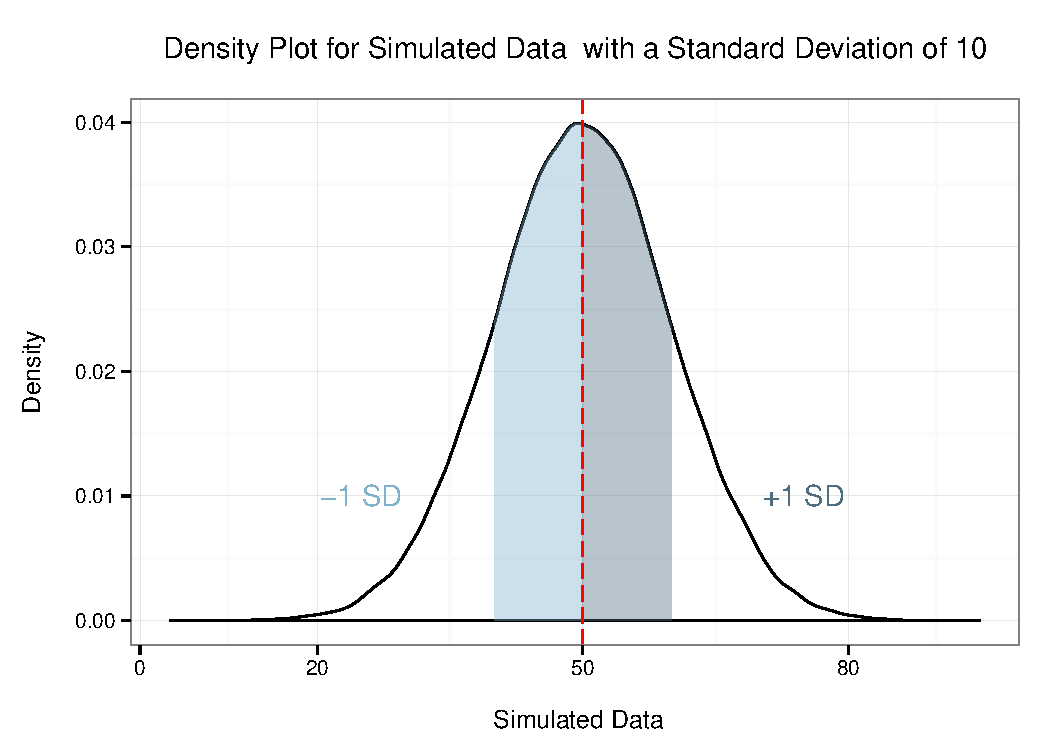
\includegraphics[width=\maxwidth]{figure/SDNormal10} 

}


\end{knitrout}

\end{frame}

% Standard deviation plot for normally distributed data with SD of 30
\begin{frame}[fragile]
\begin{knitrout}
\definecolor{shadecolor}{rgb}{0.969, 0.969, 0.969}\color{fgcolor}\begin{kframe}
\begin{alltt}
\hlcomment{# Simulate Normally Distributed data with SD of}
\hlcomment{# 30}
Normal30 <- \hlfunctioncall{rnorm}(1e+05, mean = 50, sd = 30)
\end{alltt}
\end{kframe}
\end{knitrout}


\begin{knitrout}
\definecolor{shadecolor}{rgb}{0.969, 0.969, 0.969}\color{fgcolor}

{\centering 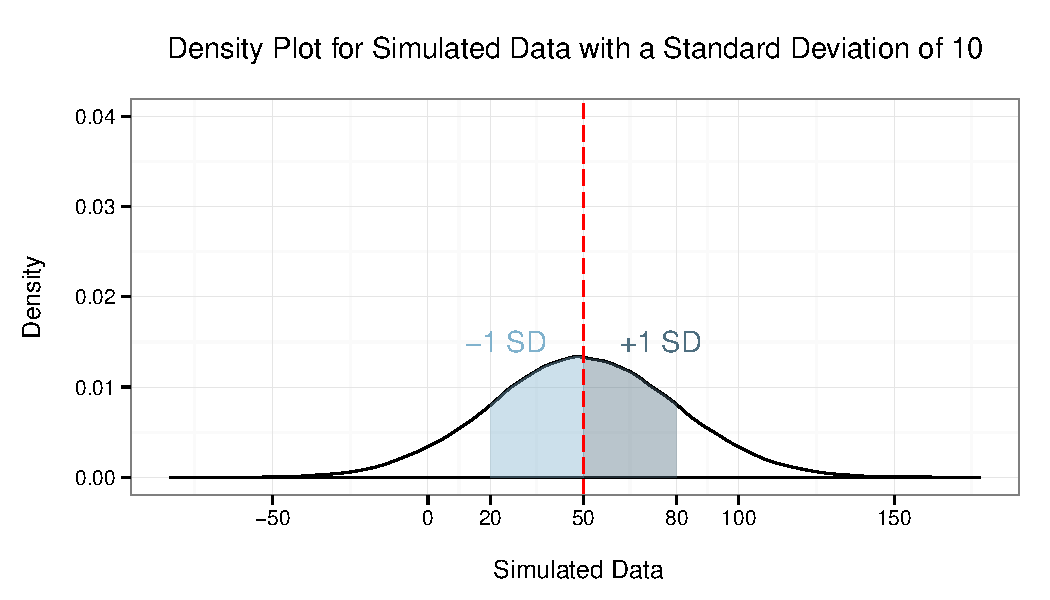
\includegraphics[width=\maxwidth]{figure/SDNormal30} 

}


\end{knitrout}

\end{frame}


\begin{frame}[fragile]
\begin{knitrout}
\definecolor{shadecolor}{rgb}{0.969, 0.969, 0.969}\color{fgcolor}

{\centering 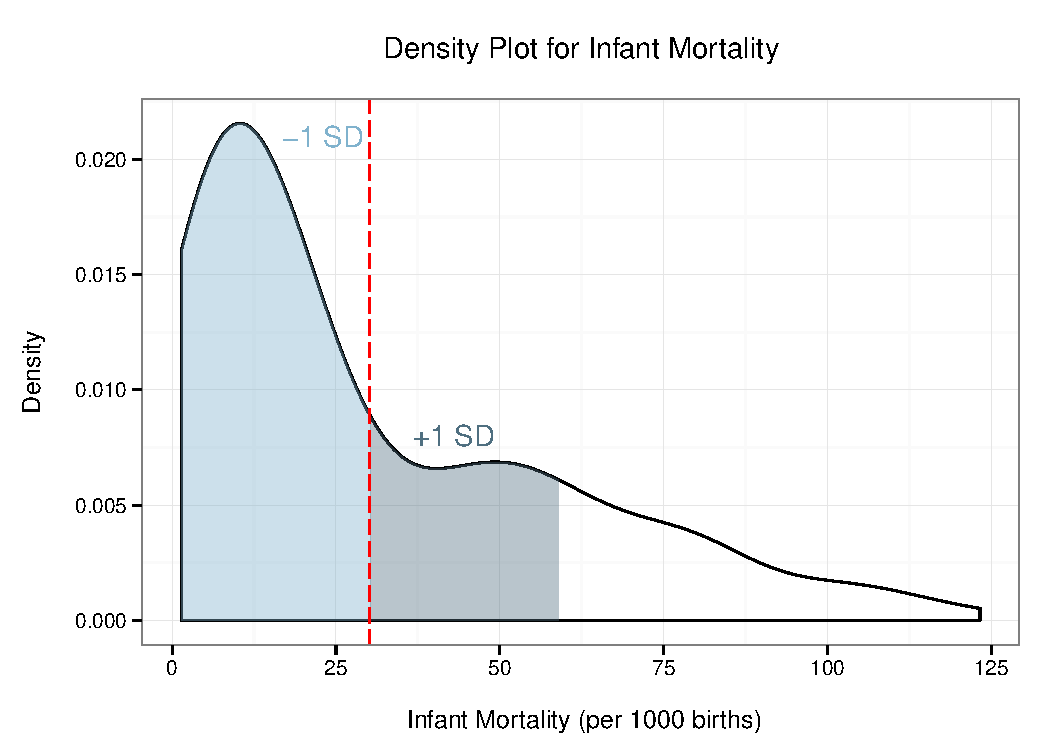
\includegraphics[width=\maxwidth]{figure/SDMort} 

}


\end{knitrout}

\end{frame}

\frame{
  \frametitle{Transforming Data}
  {\bf{Transforming Data}} \\[0.5cm]
  Transforming data can make {\bf{highly skewed}} data easier to work with. \\[0.25cm]
  Transforming data just means to {\bf{rescale}} the data using some function.\\[0.5cm]
  For example, we can {\bf{log-transform}} our Infant Mortality data to see the relationship between the two variables better.
}

\begin{frame}[fragile,plain]
\begin{knitrout}
\definecolor{shadecolor}{rgb}{0.969, 0.969, 0.969}\color{fgcolor}\begin{kframe}
\begin{alltt}
\hlcomment{# Log Transform InfantMortality}
InfantNoMiss$logInf <- \hlfunctioncall{log}(
                        InfantNoMiss$InfantMortality)
\end{alltt}
\end{kframe}
\end{knitrout}


\begin{knitrout}
\definecolor{shadecolor}{rgb}{0.969, 0.969, 0.969}\color{fgcolor}

{\centering 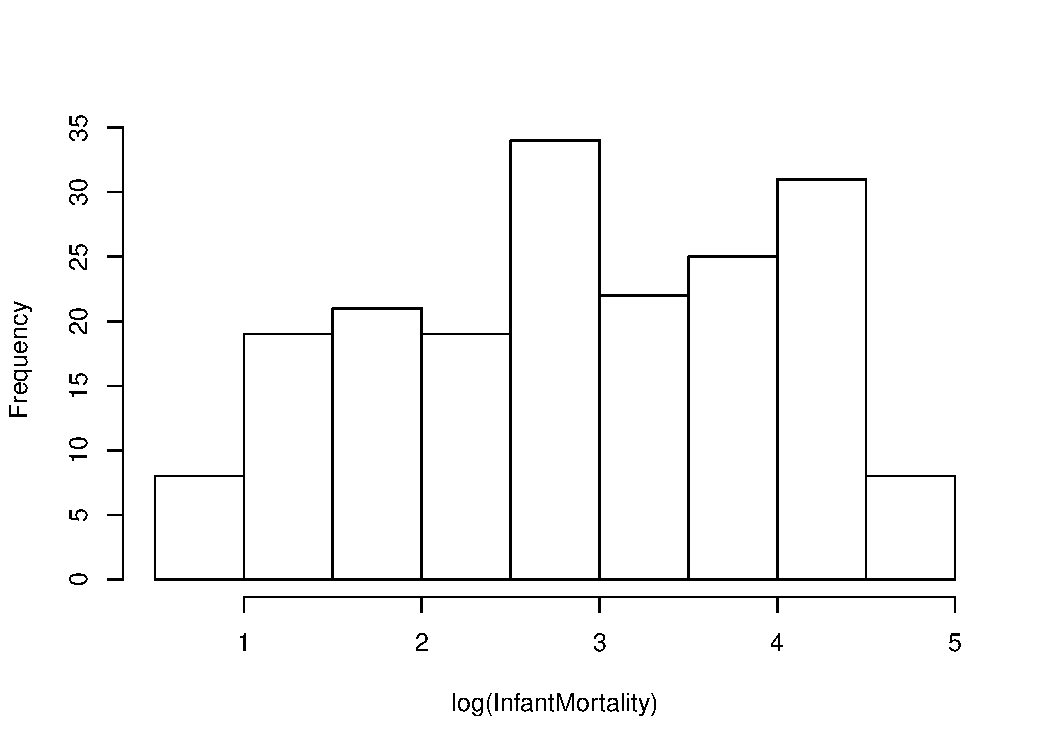
\includegraphics[width=\maxwidth]{figure/LogTransformScatter} 

}


\end{knitrout}

\end{frame}

\begin{frame}[fragile]
  \frametitle{Preview!}
\begin{knitrout}
\definecolor{shadecolor}{rgb}{0.969, 0.969, 0.969}\color{fgcolor}

{\centering 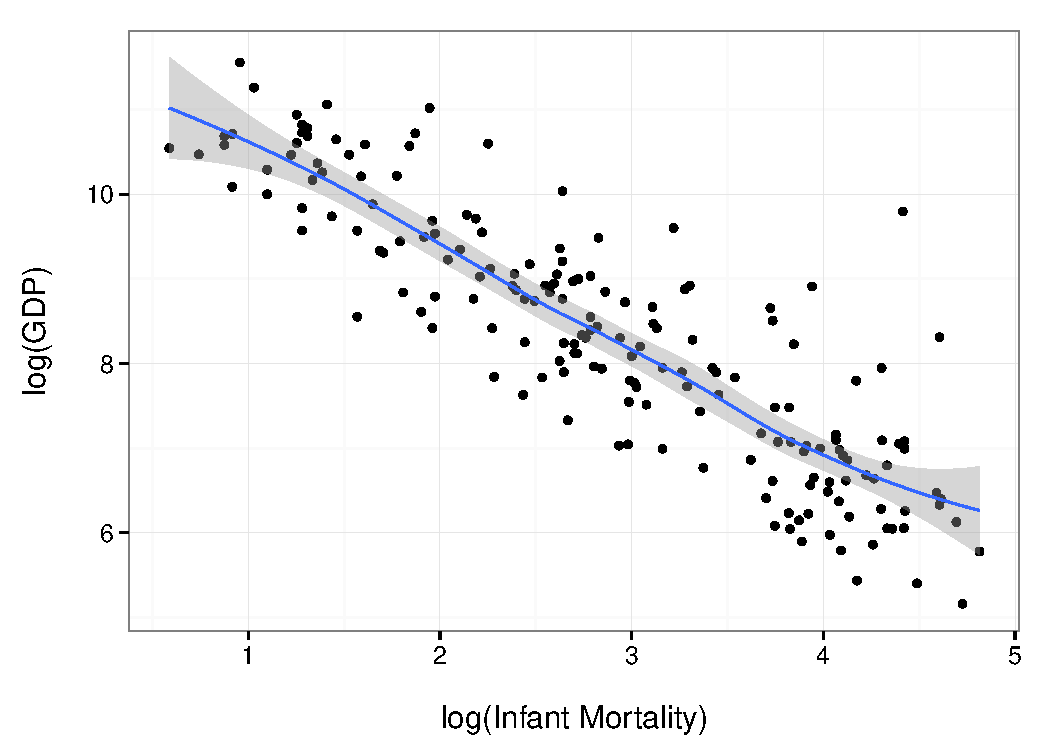
\includegraphics[width=\maxwidth]{figure/ScatterTransformed} 

}


\end{knitrout}

\end{frame}





%%%%%%%%%%%%%%%%%%%% Describing Categorical Data %%%%%%%%%%%%%%%%%%
\section{Describing Categorical Data}
\frame{
  \begin{center}
    {\LARGE{Describing Categorical Data}}
  \end{center}
}

\frame{
  \frametitle{Question}
  {\LARGE{What descriptive statistics can you use for:}}
  \begin{itemize}
    \item Ordinal data
    \item Categorical data
  \end{itemize}
}

\frame{
  \frametitle{Descriptive Statistics Catergorical Data}
  {\LARGE{You can use}}
  \begin{itemize}
    \item Ordinal data; mode, median, range, interquartile range
    \item Categorical data: mode, frequency tables/barplots
  \end{itemize}
}

\begin{frame}[fragile,plain]
\begin{knitrout}
\definecolor{shadecolor}{rgb}{0.969, 0.969, 0.969}\color{fgcolor}\begin{kframe}
\begin{alltt}
\hlcomment{# Use cars data, loaded in R by default}
\hlcomment{# Create bar plot}
\hlfunctioncall{plot}(MortalityGDP$region, xlab = \hlstring{"Region"})
\end{alltt}
\end{kframe}

{\centering 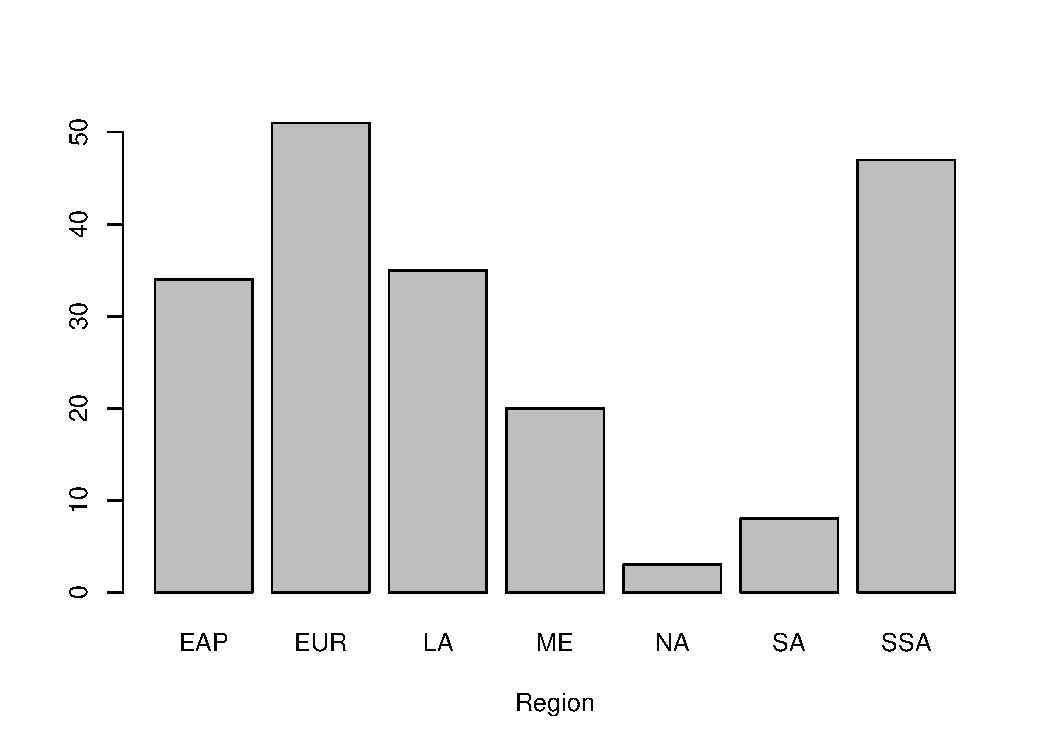
\includegraphics[width=\maxwidth]{figure/CarsBarPlot} 

}


\end{knitrout}

\end{frame}

\begin{frame}[fragile]
  \frametitle{Scatterplot-like Options for Categorical Data}
  {\Large{You can use {\bf{contingency tables}} and {\bf{mosaic plots}} like scatter plots when you have categorical data.}}
\end{frame}  

\begin{frame}[fragile,plain]
\begin{knitrout}
\definecolor{shadecolor}{rgb}{0.969, 0.969, 0.969}\color{fgcolor}\begin{kframe}
\begin{alltt}
\hlcomment{# Create High/Low Income Variable}
InfantNoMiss$DumMort[InfantNoMiss$InfantMortality
                     >= 15] <- \hlstring{"high"}
InfantNoMiss$DumMort[InfantNoMiss$InfantMortality
                     < 15] <- \hlstring{"low"}
\hlcomment{# Create contingency table}
\hlfunctioncall{table}(InfantNoMiss$region, InfantNoMiss$DumMort)
\end{alltt}
\begin{verbatim}
##      
##       high low
##   EAP   16  12
##   EUR    8  41
##   LA    20  13
##   ME     9  11
##   NA     0   2
##   SA     6   2
##   SSA   45   2
\end{verbatim}
\end{kframe}
\end{knitrout}

\end{frame}

\begin{frame}[fragile,plain]
\begin{knitrout}
\definecolor{shadecolor}{rgb}{0.969, 0.969, 0.969}\color{fgcolor}\begin{kframe}
\begin{alltt}
\hlfunctioncall{mosaicplot}(\hlfunctioncall{table}(InfantNoMiss$region, 
            InfantNoMiss$DumMort),
            main = \hlstring{"MosaicPlot: Infant Mort. & Reg."})
\end{alltt}
\end{kframe}

{\centering 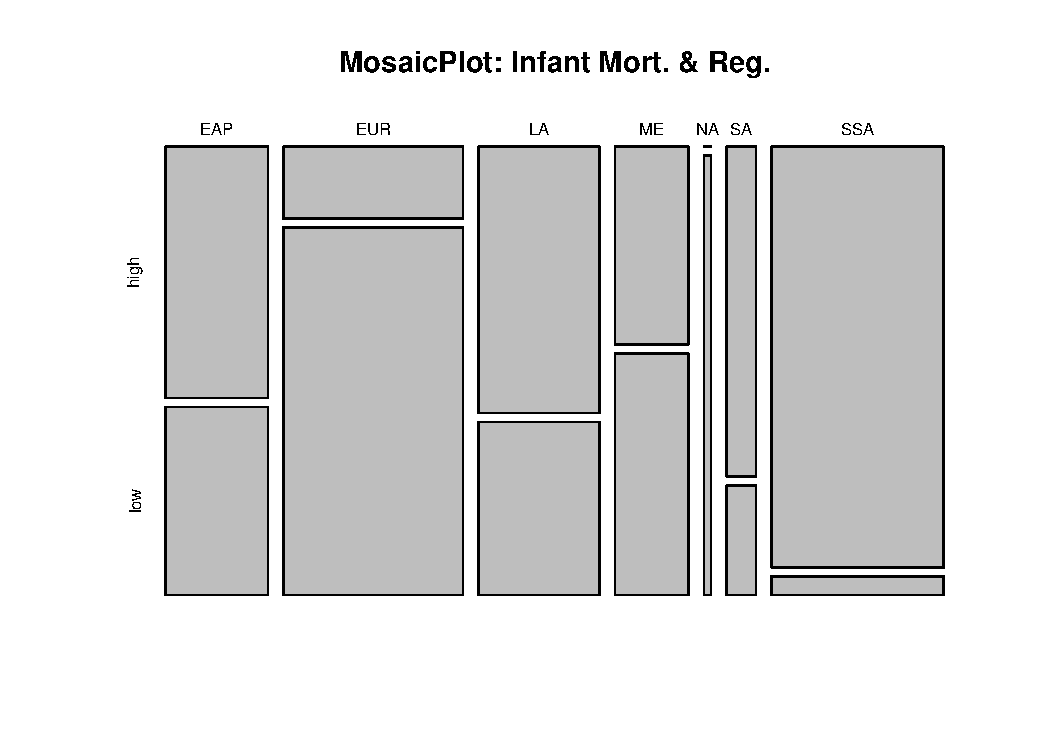
\includegraphics[width=\maxwidth]{figure/MoasicPlot} 

}


\end{knitrout}

\end{frame}

%%%%%%%% References
\begin{frame}[allowframebreaks]
  \frametitle{References}
  Crawley, Michael J. 2005. Statistics: An Introduction Using R. Chichester: John Wiley & Sons. Ltd. \\[0.25cm]
  Diaz, David M., Christopher D. Barr, and Mine \c{C}etinkaya-Rundel. OpenIntro Statistics. 1st ed. \url{http://www.openintro.org/stat/downloads.php}. \\[0.25cm] 
\end{frame}

\end{document}
